\documentclass[a4paper]{article}

\usepackage{listings}
\usepackage{color}
\usepackage{graphicx}

\usepackage[top=2.0cm, bottom=2.0cm, left=2.0cm, right=2.0cm]{geometry}

\begin{document}

\title{Embbeded Systems - Exercise 01}

\author{Jander Nascimento}

%\maketitle

Author: Jander Nascimento

\section{Part 1}

\subsection{Model}
     
	Figure represents the Kripke structure.
    
	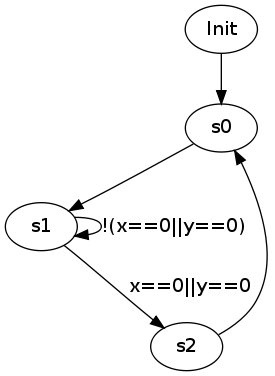
\includegraphics[scale=0.50]{final}
	
\subsection{Formulas}

Formulas tested:

	Passed formulas:
	
	\begin{itemize}
		\item $EG(!(states=s2))$
		\item $EX(state=s1)$
	\end{itemize}
	
	Failed formulas:
	\begin{itemize}
		\item $E(state=s1 U state=s2)$
		\item $E(y=0 * state=s2)$
	\end{itemize}
	
\section{Part 2}	
	
\subsection{Question 1}

\begin{lstlisting}
EF(position[0:1]=0);
EF(position[0:1]=1);
EF(position[0:1]=2);
EF(position[0:1]=3);
\end{lstlisting}

\subsection{Question 2}

\begin{lstlisting}
module elevator(position,clk,button0,button1,button2,button3);
       input clk;
       input button0, button1, button2, button3;
       output position;
       reg [1:0] position;
       reg [3:0] pressed;
       initial begin
        position = 0;
        pressed = 4;
       end

       always @(posedge clk) begin

       pressed=button0+button1+button2+button3; //create this reg so we can use in CTL

		if (button0) begin
           if (position == 0)
             pressed = 4;
           else if (position > 0)
             position = position - 1;
         end

         if (button1) begin
           if (position == 1)
             pressed = 4;
           else if (position < 1)
             position = position + 1;
           else if (position > 1)
             position = position - 1;
         end

         if (button2) begin
           if (position == 2)
             pressed = 4;
           else if (position < 2)
             position = position + 1;
           else if (position > 2)
             position = position - 1;
         end

         if (button3) begin
           if (position == 3)
             pressed = 4;
           else if (position < 3)
             position = position + 1;
         end

       end
endmodule
\end{lstlisting}

\subsection{Question 3}

//No idea, chain the state (related the current state with the previous one) without modify the code at this point :-S

\subsection{Question 4}

$EF(pressed[2:0]=2 * position[0:1]=2);$

\end{document}
